\subsection{Model Dynamics}
\label{sec:state.og.dynamics}

We are interested in the dynamics of the original model with fixed parameters $\beta = 1, f = 150, L = 4.2 \cdot 10^{-3}, R = 2, V_m = 5,$ and $\mu = 0.5$.
The parameters $E_0$ and $\chi_0$ are varied in the ranges $[14, 28]$ and $[0.1, 0.65]$, respectively.
Scanning this parameter plane for the period of stable cycles results in \Cref{fig:state.og.dynamics.period}.

\begin{figure}
	\centering
	\includegraphics[width=0.6\textwidth]{99_Yunus/2D_Period_Zoomed/result.png}
	\caption[2D scan of the periods in the original model]{
		2D scan of the periods in the original model.
		The parameters $\beta = 1, f = 150, L = 4.2 \cdot 10^{-3}, R = 2, V_m = 5,$ and $\mu = 0.5$ are fixed.
		The parameters $E_0$ and $\chi_0$ are varied in the ranges $[14, 28]$ and $[0.1, 0.65]$, respectively.
		Each color represents a different period, where lighter colors \hl{correspond to} higher periods.
		The numbers in the picture are the period of the corresponding chain of parameter regions.
		The three points $A, B,$ and $C$ mark the parameter values for the cobweb diagrams in \Cref{fig:state.og.dynamics.cobwebs}.
	}
	\label{fig:state.og.dynamics.period}
\end{figure}

The colors in the 2D scan \Cref{fig:state.og.dynamics.period} indicate the period of the stable cycle in those regions.
Brighter colors \hl{correspond to} higher periods.
Points $A, B$ and $C$ are in the parameter region, which has stable cycles with the period 12.
\hl{The parameter regions differ in another way, the cycles in these regions are associated with different symbolic sequences}.
As mentioned before, it describes on which branches of the model function the points of the cycle exist.
Some cobweb diagrams illustrate the difference between the parameter regions.

\begin{align}
	F(\theta + \pi) \equiv F(\theta) + \pi \mod 2\pi \label{equ:state.og.sym}
\end{align}

\Citeauthor{akyuz2022} pointed out a symmetry in the original model.
\Cref{equ:state.og.sym} describes this symmetry~\cite{akyuz2022}.
This means that the shapes of the branches $F_\A$ and $F_\C$ are identical.
The branch $F_\C$ is exactly $\pi$ to the right of $F_\A$ and its values are $\pi$ larger.
The same is true for the branches $F_\B$ and $F_\D$.
It follows that if $x$ is a part of a cycle in the original model, the point $x + \pi$ belongs to a cycle as well.
Therefore, only the two following cases are possible:

\begin{enumerate}[label=(\Alph*)]
	\item The points $x$ and $x + \pi$ belong to the same cycle.
	      This cycle is therefore symmetric, and we will refer to such cycles as ``type A'' cycles.
	      Such cycles must have an even period because there are as many points on the intervals $I_\A$ and $I_\B$ as there are on the intervals $I_\C$ and $I_\D$.
	\item The points $x$ and $x + \pi$ belong to different cycles.
	      Then there are at least 2 coexisting cycles with the same period.
	      This is not obvious and therefore proven below. %in \Cref{proof:state.cycle.B.coex}.
	      We will call these cycles ``type B'' cycles.
\end{enumerate}

\begin{proof}[At Least Two Coexisting ``Type B'' Cycles] \phantom{x} \\
	Let $\O_k = \left\{x_i \:\mid\: 0 \leq i < k\right\}$ be a $k$-cycle of the original model where $x_i + \pi \not\in O_k$ for some $0 \leq i < k$.
	It follows that $x_i + \pi \not\in \O_k$ for any $x_i \in \O_k$.
	%If for some $x_i \in \O_k$ the image of $x_i + \pi$ was in the cycle $F(x_i + \pi) \in \O_k$ then $x_i + \pi$ must also be in the cycle, since $F^{k-1}\left(F\left(x_i + \pi\right)\right) = F^k\left(x_i + \pi\right) = x_i + \pi$.

	Then there is a second cycle $\O'_k = \left\{x_i + \pi \:\mid\: x_i \in \O_k\right\}$.
	This cycle $\O'_k$ is completely disjunct from the first cycle $\O_k$ per definition.
	Therefore, there are at least two coexisting cycles $\O_k \neq \O'_k$ with the same period. \hfill	$\blacksquare$
\end{proof}

\Cref{fig:state.og.dynamics.cobwebs} shows the cobweb diagrams at points $A$ and $C$.
Both parameter regions have only one stable cycle of period 12.
The stable cycle at point $A$ has the symbolic sequence $\A^3\B^3\C^3\D^3$ and the cycle at point $C$ has the symbolic sequence $\A^2\B^4\C^2\D^4$.
We follow the convention, that the branch with the smallest positive boundaries is called branch $\A$.
And the next one branch $\B$ and so on.

\Cref{fig:state.og.dynamics.cobweb.B} shows the cobweb diagram at point $B$.
By looking closely, one can see that there are 2 coexisting cycles in this cobweb diagram.
One cycle has the symbolic sequence $\A^3\B^3\C^2\D^4$, while the other one has the symbolic sequence $\A^2\B^2\C^3\D^3$.
Both cycles are asymmetric.
And they are similar to each other in the way that $\Cycle{\A^3\B^3\C^2\D^4}$ behaves on the branches $\A$ and $\B$ like $\Cycle{\A^2\B^2\C^3\D^3}$ on the branches $\C$ and $\D$ and vice versa.
One can think of the cycles being equivalent by shifting them by $\pi$ in either direction.
Due to the symmetry of the model, an asymmetric stable cycle necessarily must exist alongside another asymmetric stable cycle that is itself, but shifted by $\pi$.
These cycles also behave similarly to both the cycles at points $A$ and $B$.
The cycle $\Cycle{\A^3\B^3\C^2\D^4}$ behaves like the cycle $\Cycle{\A^3\B^3\C^3\D^3}$ at point $A$ on its left half, while it behaves like the cycle $\Cycle{\A^2\B^4\C^2\D^4}$ on its right half.
The same is true for the cycle $\Cycle{\A^2\B^4\C^3\D^3}$ but reversed since it is the other cycle shifted by $\pi$.
We call the previously described parameter regions with only one symmetrical stable cycle ``type A'' parameter regions.
The just described parameter regions with 2 asymmetrical coexisting cycles will be called ``type B'' parameter regions.

\begin{figure}
	\centering
	\begin{subfigure}{0.3\textwidth}
		\centering
		\includegraphics[width=\textwidth]{99_Yunus/Period12/Cobweb_A_12/result.png}
		\caption{At point $A$}
		\label{fig:state.og.dynamics.cobweb.A}
	\end{subfigure}
	\begin{subfigure}{0.3\textwidth}
		\centering
		\includegraphics[width=\textwidth]{99_Yunus/Period12/Cobweb_B_12/Manual/result.png}
		\caption{At point $B$}
		\label{fig:state.og.dynamics.cobweb.B}
	\end{subfigure}
	\begin{subfigure}{0.3\textwidth}
		\centering
		\includegraphics[width=\textwidth]{99_Yunus/Period12/Cobweb_C_12/result.png}
		\caption{At point $C$}
		\label{fig:state.og.dynamics.cobweb.C}
	\end{subfigure}
	\caption[Cobweb diagrams of the original model]{
		Cobweb diagrams at three values of the parameters $E_0$ and $\chi_0$ in the original model with fixed parameters $\beta = 1, f = 150, L = 4.2 \cdot 10^{-3}, R = 2, V_m = 5,$ and $\mu = 0.5$.
		The parameter values of $E_0$ and $\chi_0$ are marked in \Cref{fig:state.og.dynamics.period}.
		(a) shows the cycle $\Cycle{\A^3\B^3\C^3\D^3}$ at point $A$, (b) shows the two coexisting cycles $\Cycle{\A^3\B^3\C^2\D^4}$ (green) and $\Cycle{\A^2\B^4\C^3\D^3}$ (red) at point $B$, and (c) shows the cycle $\Cycle{\A^2\B^4\C^2\D^4}$ at point $C$.
	}
	\label{fig:state.og.dynamics.cobwebs}
\end{figure}

This behavior is peculiar.
To summarize, we have chains of parameter regions with the same period.
The type of the parameter regions alternates between ``type A'' and ``type B''.
When the stable cycle in one ``type A'' parameter region is $\Cycle{\A^a\B^b\C^a\D^b}$, the stable cycle in the next ``type A'' parameter region is $\Cycle{\A^{c}\B^{d}\C^{c}\D^{d}}$ with $c = a - 1$ and $d = b + 1$.
The ``type B'' parameter region in between two ``type A'' parameter regions of a chain with cycles $\Cycle{\A^a\B^b\C^c\D^d}$ and $\Cycle{\A^{c}\B^{d}\C^{a}\D^{b}}$, has the two cycles $\Cycle{\A^x\B^y\C^{x-1}\D^{y+1}}$ and $\Cycle{\A^{x-1}\B^{y+1}\C^x\D^y}$.
Also, there is not only one chain, but many chains next to each other where the period increases by 2 from one chain to the next.
